%%%%%%%%%%%%%%%%%%%%%%%%%%%%%%%%%%%%%%%%%%%%%%%%%%%%%%%%%%%%%%%%%%%%%%%%%%%

\documentclass{standalone}

\usepackage{amsmath}
\usepackage{mathptmx}
\usepackage{pgfplots}
\usetikzlibrary{external}
\tikzexternalize{interest-quarterly}
\pgfplotsset{compat=1.15}

%% IEEE uses Times Roman font, so we'll default to Times.
%% These three commands make up the entire times.sty package.
\renewcommand{\rmdefault}{ptm}
\renewcommand{\ttdefault}{pcr}
\normalfont\selectfont

\begin{document}

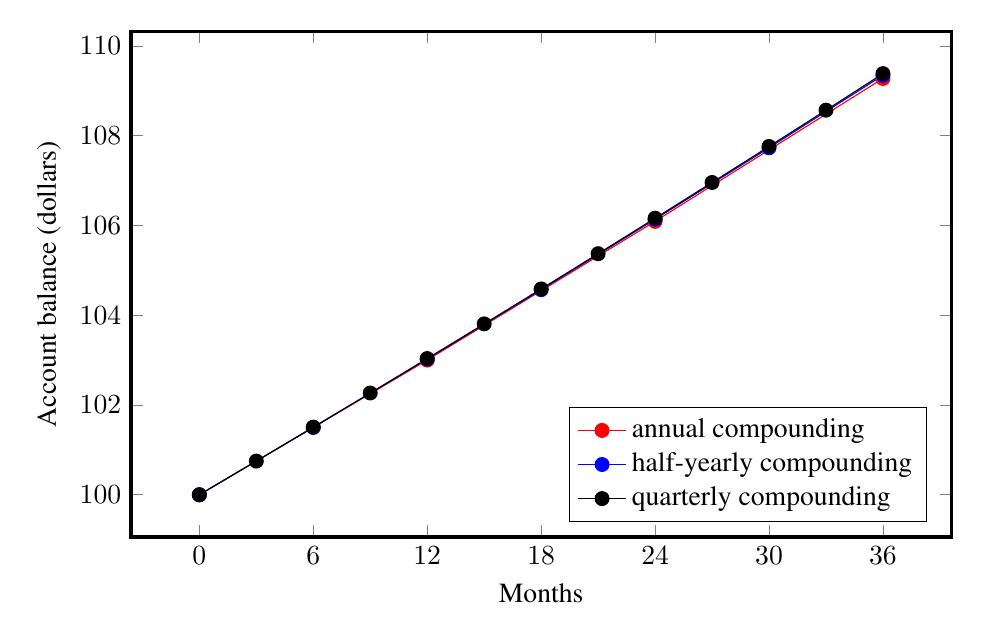
\begin{tikzpicture}
\tikzset{%%
  every mark/.append style={scale=1.0},%%
  scale=1.0%%
}
\pgfplotsset{%%
  every axis/.append style={font=\normalsize}%%
}
%%
\begin{axis}[%%
  axis line style=very thick,%%
  dotBlackStyle/.style={mark size=2.5,black,mark color=black,mark=*},%%
  dotBlueStyle/.style={mark size=2.5,blue,mark color=blue,mark=*},%%
  dotRedStyle/.style={mark size=2.5,red,mark color=red,mark=*},%%
  enlargelimits=true,%%
  height=8cm,%%
  legend cell align=left,%%
  legend pos=south east,%%
  plotStyle/.style={%%
    domain=4:17,%%
    mark=none,%%
    smooth,%%
    thick%%
  },%%
  width=12cm,%%
  %% x axis
  xlabel={\normalsize Months},%%
  xtick={0,6,12,18,24,30,36},%%
  xticklabels={$0$,$6$,$12$,$18$,$24$,$30$,$36$},%%
  %% y axis
  ylabel={\normalsize Account balance~(dollars)},%%
  scaled y ticks=false,%%
  y tick label style=/pgf/number format/fixed%%
]
%%
%%
\addplot[dotRedStyle] coordinates {
  (0, 100.000000)
  (12, 103.000000)
  (24, 106.090000)
  (36, 109.272700)
};
\addlegendentry{annual compounding}
%%
%%
\addplot[dotBlueStyle] coordinates {
  (0, 100.000000)
  (6, 101.500000)
  (12, 103.022500)
  (18, 104.567837)
  (24, 106.136355)
  (30, 107.728400)
  (36, 109.344326)
};
\addlegendentry{half-yearly compounding}
%%
%%
\addplot[dotBlackStyle] coordinates {
  (0, 100.000000)
  (3, 100.750000)
  (6, 101.505625)
  (9, 102.266917)
  (12, 103.033919)
  (15, 103.806673)
  (18, 104.585224)
  (21, 105.369613)
  (24, 106.159885)
  (27, 106.956084)
  (30, 107.758255)
  (33, 108.566441)
  (36, 109.380690)
};
\addlegendentry{quarterly compounding}
\end{axis}
\end{tikzpicture}

\end{document}
